\hypertarget{tenduxeancias-cloud-scada-e-digital-twin}{%
\chapter{Tendências: Cloud SCADA e Digital Twin}\label{tenduxeancias-cloud-scada-e-digital-twin}}

\section*{Objetivos de Aprendizagem}

Ao final deste capítulo, o leitor será capaz de:

\begin{itemize}
\tightlist
\item
  Descrever as vantagens e desafios do Cloud SCADA versus SCADA on-premises.
\item
  Identificar as principais plataformas de Cloud SCADA disponíveis no mercado.
\item
  Compreender como o Digital Twin se integra aos sistemas SCADA para otimização.
\item
  Analisar o impacto da IA/ML e do low-code/no-code no futuro dos sistemas supervisórios.
\end{itemize}

\begin{center}\rule{0.5\linewidth}{0.5pt}\end{center}

\hypertarget{cloud-scada-conceito-e-motivauxe7uxf5es}{%
\section{Cloud SCADA: Conceito e Motivações}\label{cloud-scada-conceito-e-motivauxe7uxf5es}}

O \textbf{Cloud SCADA} é a evolução natural dos sistemas supervisórios tradicionais: em vez de servidores físicos instalados na própria planta (\emph{on-premises}), o software SCADA é hospedado em infraestrutura de nuvem pública (AWS, Azure, Google Cloud) ou privada.

\hypertarget{por-que-migrar-para-a-nuvem}{%
\subsection{Por que migrar para a nuvem?}\label{por-que-migrar-para-a-nuvem}}

\textbf{Tabela 9.1 -- SCADA On-Premises \ensuremath{\times} Cloud SCADA}

\begin{longtable}[]{@{}
  >{\raggedright\arraybackslash}p{(\columnwidth - 4\tabcolsep) * \real{0.3333}}
  >{\raggedright\arraybackslash}p{(\columnwidth - 4\tabcolsep) * \real{0.3333}}
  >{\raggedright\arraybackslash}p{(\columnwidth - 4\tabcolsep) * \real{0.3333}}@{}}
\toprule\noalign{}
\begin{minipage}[b]{\linewidth}\raggedright
Critério
\end{minipage} & \begin{minipage}[b]{\linewidth}\raggedright
SCADA On-Premises
\end{minipage} & \begin{minipage}[b]{\linewidth}\raggedright
Cloud SCADA
\end{minipage} \\
\midrule\noalign{}
\endhead
\bottomrule\noalign{}
\endlastfoot
\textbf{Infraestrutura} & Servidores físicos na planta & Instâncias virtuais gerenciadas \\
\textbf{Custo inicial (CapEx)} & Alto (hardware + licenças) & Baixo ou zero \\
\textbf{Custo operacional (OpEx)} & Equipe de TI, manutenção, energia & Pagamento por uso (pay-as-you-go) \\
\textbf{Escalabilidade} & Limitada (hardware físico) & Elástica (escala automaticamente) \\
\textbf{Acesso remoto} & Via VPN, complexo & Nativo via browser, global \\
\textbf{Atualizações} & Manual, risco de incompatibilidade & Automáticas, sem downtime \\
\textbf{Latência} & Mínima (rede local) & Depende da conectividade WAN \\
\textbf{Disponibilidade garantida} & Depende do investimento local & SLAs de 99,9\% a 99,99\% \\
\textbf{Compliance / Soberania de dados} & Total controle & Depende da região do datacenter \\
\end{longtable}

\hypertarget{arquitetura-cloud-scada}{%
\subsection{Arquitetura Cloud SCADA}\label{arquitetura-cloud-scada}}

\begin{center}
\IfFileExists{../figuras/capitulo-09-m1.pdf}{%
  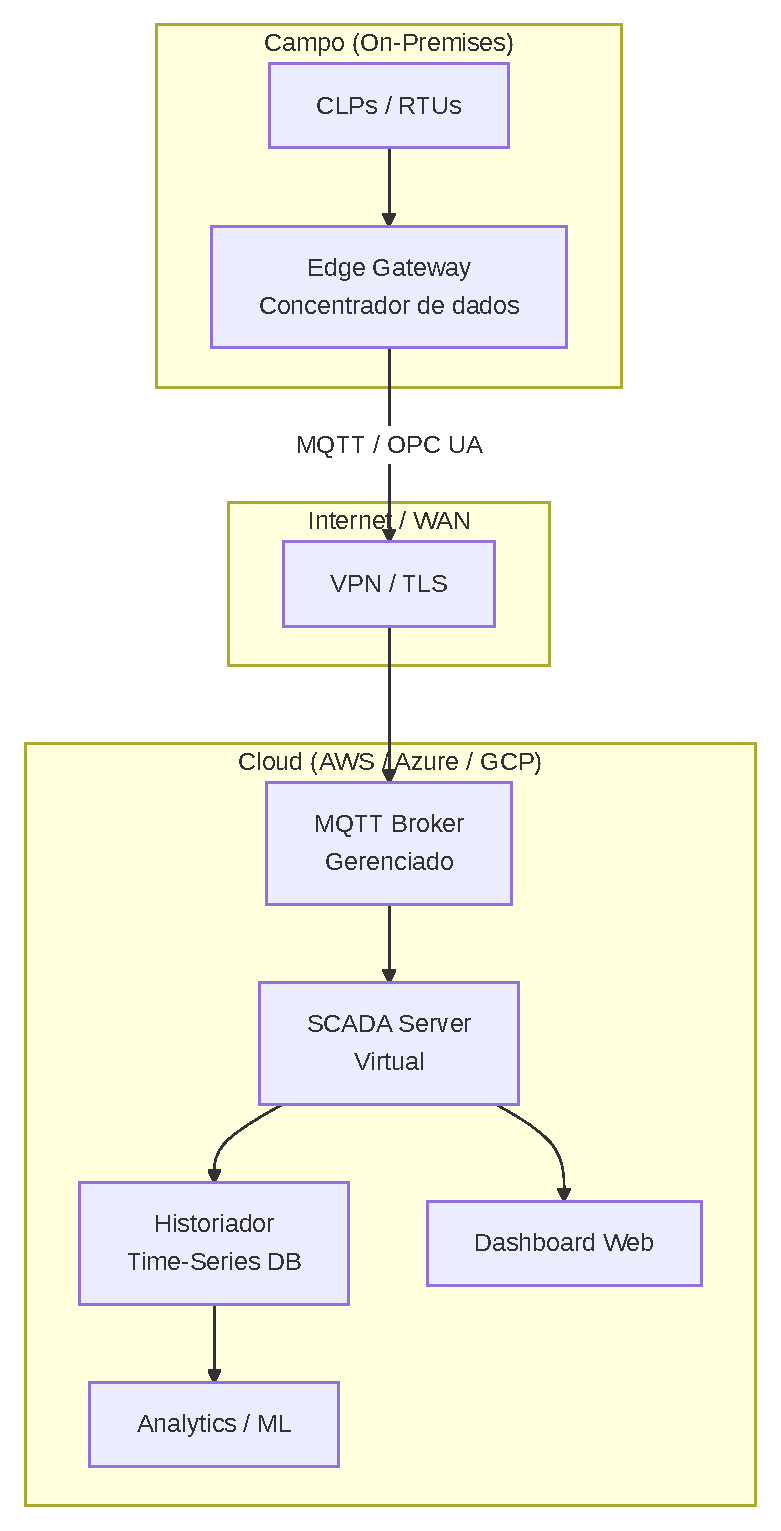
\includegraphics[width=\linewidth,height=0.8\textheight,keepaspectratio]{../figuras/capitulo-09-m1.pdf}%
}{\fbox{\parbox{0.9\linewidth}{\small Diagrama Mermaid ainda não renderizado: capitulo-09-m1. Rode scripts/render-mermaid.sh.}}}
\end{center}

\begin{caixafigura}

\textbf{{[}Figura 9.1 -- Arquitetura Cloud SCADA com Edge Gateway{]}}
\emph{Diagrama colorido mostrando: (esquerda) campo industrial com CLPs e edge gateway; (centro) conexão segura via VPN/TLS pela internet; (direita) nuvem com os componentes SCADA virtualizados. Destacar que o controle em tempo real permanece no CLP local --- a nuvem é supervisão e analytics.}

\end{caixafigura}

\begin{caixaatencao}

\textbf{Atenção:} Em Cloud SCADA, o \textbf{controle em malha fechada permanece nos CLPs locais}. A latência da nuvem (decenas a centenas de ms) inviabiliza controle PID via cloud. A nuvem é responsável pela supervisão, historização, analytics e acesso remoto --- não pelo controle direto do processo.

\end{caixaatencao}

\begin{center}\rule{0.5\linewidth}{0.5pt}\end{center}

\hypertarget{plataformas-de-cloud-scada}{%
\section{Plataformas de Cloud SCADA}\label{plataformas-de-cloud-scada}}

\hypertarget{ignition-cloud-edition-inductive-automation}{%
\subsection{Ignition Cloud Edition (Inductive Automation)}\label{ignition-cloud-edition-inductive-automation}}

O \textbf{Ignition} foi pioneiro no modelo de licenciamento cloud-native:

\begin{itemize}
\tightlist
\item
  Hospedado na AWS ou Azure.
\item
  Mesma interface do Ignition on-premises --- sem curva de aprendizado adicional.
\item
  Módulo de borda (\emph{Ignition Edge}) instalado na planta coleta dados e sincroniza com a cloud.
\item
  Ideal para empresas com múltiplos sites que precisam de visão unificada.
\end{itemize}

\hypertarget{aws-iot-sitewise}{%
\subsection{AWS IoT SiteWise}\label{aws-iot-sitewise}}

O \textbf{AWS IoT SiteWise} é a solução da Amazon para modelagem e supervisão de ativos industriais:

\begin{itemize}
\tightlist
\item
  \textbf{Asset Models:} define hierarquia de ativos (planta \ensuremath{\rightarrow} unidade \ensuremath{\rightarrow} equipamento \ensuremath{\rightarrow} componente).
\item
  \textbf{Asset Properties:} variáveis de processo com cálculos e transformações configuráveis.
\item
  \textbf{SiteWise Monitor:} dashboards de supervisão sem código.
\item
  \textbf{SiteWise Edge:} módulo local para operação sem conectividade.
\end{itemize}

\hypertarget{azure-iot-hub-azure-digital-twins}{%
\subsection{Azure IoT Hub + Azure Digital Twins}\label{azure-iot-hub-azure-digital-twins}}

A combinação \textbf{Azure IoT Hub} (ingestão de dados) + \textbf{Azure Digital Twins} (modelagem) + \textbf{Azure Time Series Insights} (histórico) + \textbf{Power BI} (dashboards) forma uma stack completa de Cloud SCADA na Microsoft.

\hypertarget{aveva-insight}{%
\subsection{AVEVA Insight}\label{aveva-insight}}

O \textbf{AVEVA Insight} é a solução cloud da AVEVA (herdeira do PI System e Wonderware):

\begin{itemize}
\tightlist
\item
  Historização de dados na nuvem com a mesma interface do PI System.
\item
  KPIs e dashboards web sem necessidade de servidor local.
\item
  Integração nativa com System Platform on-premises existentes.
\end{itemize}

\begin{caixadica}

\textbf{Dica:} Para plantas industriais brasileiras com dados sensíveis de processo, verifique a conformidade com a \textbf{LGPD} (Lei Geral de Proteção de Dados) e a \textbf{soberania de dados}: dados de processo podem conter informações estratégicas. Priorize regiões de datacenter no Brasil (AWS São Paulo, Azure Brasil Sul) ou considere nuvem privada (\emph{on-premises cloud}).

\end{caixadica}

\begin{center}\rule{0.5\linewidth}{0.5pt}\end{center}

\hypertarget{digital-twin-nos-sistemas-scada}{%
\section{Digital Twin nos Sistemas SCADA}\label{digital-twin-nos-sistemas-scada}}

A integração do \textbf{Digital Twin} com o SCADA cria um sistema de supervisão que não apenas monitora --- mas também simula, prevê e otimiza.

\hypertarget{como-o-scada-alimenta-o-digital-twin}{%
\subsection{Como o SCADA alimenta o Digital Twin}\label{como-o-scada-alimenta-o-digital-twin}}

\begin{center}
\IfFileExists{../figuras/capitulo-09-m2.pdf}{%
  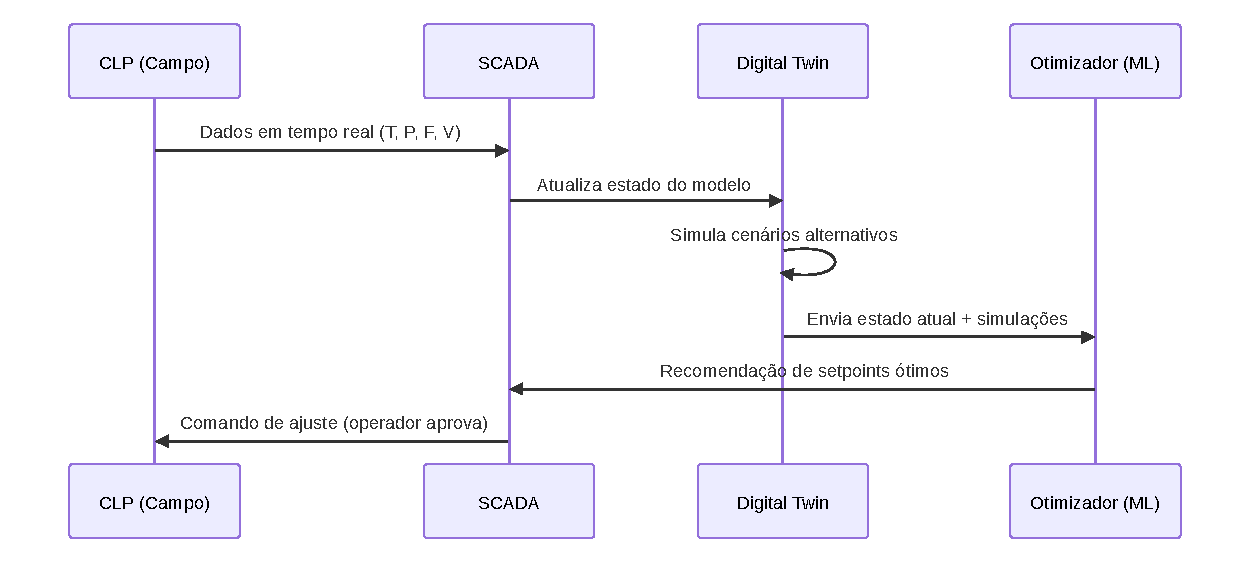
\includegraphics[width=\linewidth,height=0.8\textheight,keepaspectratio]{../figuras/capitulo-09-m2.pdf}%
}{\fbox{\parbox{0.9\linewidth}{\small Diagrama Mermaid ainda não renderizado: capitulo-09-m2. Rode scripts/render-mermaid.sh.}}}
\end{center}

\begin{caixafigura}

\textbf{{[}Figura 9.2 -- Integração SCADA e Digital Twin: ciclo de otimização{]}}
\emph{Diagrama do ciclo acima com representações visuais: planta física com sensores \ensuremath{\rightarrow} SCADA \ensuremath{\rightarrow} modelo 3D digital twin \ensuremath{\rightarrow} algoritmo de otimização \ensuremath{\rightarrow} recomendação ao operador no SCADA \ensuremath{\rightarrow} ajuste no processo real. Ciclo contínuo indicado por setas.}

\end{caixafigura}

\hypertarget{caso-de-uso-otimizauxe7uxe3o-de-destilauxe7uxe3o}{%
\subsection{Caso de Uso: Otimização de Destilação}\label{caso-de-uso-otimizauxe7uxe3o-de-destilauxe7uxe3o}}

Em uma coluna de destilação de uma refinaria, o Digital Twin permite:

\begin{enumerate}
\def\labelenumi{\arabic{enumi}.}
\tightlist
\item
  \textbf{Modelo de primeiro princípio} (equações de equilíbrio termodinâmico) calibrado com dados reais do SCADA.
\item
  Simulação em tempo real de múltiplos setpoints alternativos de temperatura e refluxo.
\item
  Identificação do ponto ótimo que maximiza rendimento do produto e minimiza consumo de energia.
\item
  Recomendação ao operador com justificativa técnica e previsão de impacto.
\end{enumerate}

\textbf{Resultado típico:} ganho de 2--5\% no rendimento do destilado com redução de 8--12\% no consumo de vapor.

\begin{center}\rule{0.5\linewidth}{0.5pt}\end{center}

\hypertarget{inteliguxeancia-artificial-aplicada-a-sistemas-supervisuxf3rios}{%
\section{Inteligência Artificial Aplicada a Sistemas Supervisórios}\label{inteliguxeancia-artificial-aplicada-a-sistemas-supervisuxf3rios}}

\hypertarget{manutenuxe7uxe3o-preditiva-pdm}{%
\subsection{Manutenção Preditiva (PdM)}\label{manutenuxe7uxe3o-preditiva-pdm}}

A \textbf{manutenção preditiva} usa modelos de ML para prever falhas antes que ocorram, com base em dados históricos e em tempo real:

\begin{longtable}[]{@{}
  >{\raggedright\arraybackslash}p{(\columnwidth - 4\tabcolsep) * \real{0.3333}}
  >{\raggedright\arraybackslash}p{(\columnwidth - 4\tabcolsep) * \real{0.3333}}
  >{\raggedright\arraybackslash}p{(\columnwidth - 4\tabcolsep) * \real{0.3333}}@{}}
\toprule\noalign{}
\begin{minipage}[b]{\linewidth}\raggedright
Algoritmo
\end{minipage} & \begin{minipage}[b]{\linewidth}\raggedright
Aplicação
\end{minipage} & \begin{minipage}[b]{\linewidth}\raggedright
Indicadores Monitorados
\end{minipage} \\
\midrule\noalign{}
\endhead
\bottomrule\noalign{}
\endlastfoot
\textbf{LSTM (Long Short-Term Memory)} & Degradação de bombas e compressores & Vibração, temperatura de mancal, corrente \\
\textbf{Isolation Forest} & Detecção de anomalias em sensores & Desvios estatísticos multivariados \\
\textbf{Random Forest} & Classificação de modo de falha & Padrões de alarmes históricos \\
\textbf{Redes Neurais Convolucionais} & Análise de vibração espectral & FFT de sinal de acelerômetro \\
\end{longtable}

\hypertarget{controle-avanuxe7ado-com-ia}{%
\subsection{Controle Avançado com IA}\label{controle-avanuxe7ado-com-ia}}

\begin{itemize}
\tightlist
\item
  \textbf{MPC} (\emph{Model Predictive Control}): controlador baseado em modelo que prevê o comportamento futuro do processo e otimiza ações de controle considerando restrições.
\item
  \textbf{RL} (\emph{Reinforcement Learning}): agente aprende a operar o processo por tentativa e erro no Digital Twin --- depois é implantado na planta real.
\end{itemize}

\hypertarget{processamento-de-linguagem-natural-nlp-em-scada}{%
\subsection{Processamento de Linguagem Natural (NLP) em SCADA}\label{processamento-de-linguagem-natural-nlp-em-scada}}

Interfaces conversacionais permitem que operadores consultem o SCADA por voz ou texto:

\begin{itemize}
\tightlist
\item
  \emph{``Qual foi a temperatura máxima do Reator 3 na última semana?''}
\item
  \emph{``Mostre o histórico de alarmes do Compressor A12 nos últimos 30 dias.''}
\item
  \emph{``Qual bomba teve o maior consumo de energia no turno da manhã?''}
\end{itemize}

\begin{center}\rule{0.5\linewidth}{0.5pt}\end{center}

\hypertarget{low-code-no-code-em-supervisuxf3rios}{%
\section{Low-Code / No-Code em Supervisórios}\label{low-code-no-code-em-supervisuxf3rios}}

A tendência \textbf{low-code/no-code} está democratizando o desenvolvimento de sistemas supervisórios:

\begin{longtable}[]{@{}
  >{\raggedright\arraybackslash}p{(\columnwidth - 4\tabcolsep) * \real{0.3333}}
  >{\raggedright\arraybackslash}p{(\columnwidth - 4\tabcolsep) * \real{0.3333}}
  >{\raggedright\arraybackslash}p{(\columnwidth - 4\tabcolsep) * \real{0.3333}}@{}}
\toprule\noalign{}
\begin{minipage}[b]{\linewidth}\raggedright
Plataforma
\end{minipage} & \begin{minipage}[b]{\linewidth}\raggedright
Abordagem
\end{minipage} & \begin{minipage}[b]{\linewidth}\raggedright
Ideal para
\end{minipage} \\
\midrule\noalign{}
\endhead
\bottomrule\noalign{}
\endlastfoot
\textbf{Ignition} & Configuração por objetos, scripts Python/Jython & Integradores e engenheiros de automação \\
\textbf{Node-RED} & Flow-based visual, zero código & Prototipagem, técnicos, pequenas plantas \\
\textbf{AWS IoT SiteWise Monitor} & Dashboards sem código & Operadores, gerentes de planta \\
\textbf{Microsoft Power Apps + Power BI} & Low-code apps e dashboards & Integração com dados industriais no Office 365 \\
\textbf{Grafana} & Configuração visual de dashboards & Analytics, visualização avançada \\
\end{longtable}

\begin{caixafigura}

\textbf{{[}Figura 9.3 -- Espectro low-code / no-code em supervisórios{]}}
\emph{Gráfico de eixo horizontal: de ``No-Code'' (esquerda) a ``Full-Code'' (direita). Posicionar as ferramentas: AWS SiteWise Monitor e Power BI (no-code), Node-RED e Grafana (low-code), Ignition (low-code/code), AVEVA System Platform e Honeywell Experion (code intensivo). Eixo vertical: nível de customização \ensuremath{\times} complexidade.}

\end{caixafigura}

\begin{center}\rule{0.5\linewidth}{0.5pt}\end{center}

\hypertarget{o-futuro-da-profissuxe3o-converguxeancia-tiot}{%
\section{O Futuro da Profissão: Convergência TI/OT}\label{o-futuro-da-profissuxe3o-converguxeancia-tiot}}

O engenheiro de automação do futuro precisa transitar entre dois mundos:

\textbf{Competências OT (tradicionais):}
- Instrumentação e controle de processo (PID, cascata, ratio).
- Programação de CLPs (IEC 61131-3).
- Redes industriais (Modbus, Profibus, PROFINET).
- Normas de segurança funcional (IEC 61511, IEC 61508).

\textbf{Competências TI (emergentes):}
- Redes TCP/IP, cloud computing.
- Protocolos IIoT (MQTT, OPC UA, REST).
- Análise de dados (Python, pandas, scikit-learn).
- Cibersegurança industrial (IEC 62443).
- DevOps industrial: containers (Docker), CI/CD para automação.

\begin{caixafigura}

\textbf{{[}Figura 9.4 -- Roadmap de evolução do SCADA: dos anos 1970 ao futuro{]}}
\emph{Linha do tempo em perspectiva: (1970s) SCADA monolítico com mainframe; (1980s) sistemas proprietários distribuídos; (1990s) Ethernet + OPC; (2000s) SCADA em rede TCP/IP; (2010s) IIoT + cloud; (2020s) AI-SCADA + Digital Twin + 5G; (2030s?) Autonomous Operations. Ícones de tela de cada era.}

\end{caixafigura}

\begin{center}\rule{0.5\linewidth}{0.5pt}\end{center}

\hypertarget{estudo-de-caso-piloto-de-cloud-scada-em-uma-frota-de-elevatuxf3rias}{%
\section{\texorpdfstring{Estudo de Caso --- Piloto de Cloud SCADA em uma frota de elevatórias}{Estudo de Caso  Piloto de Cloud SCADA em uma frota de elevatórias}}\label{estudo-de-caso-piloto-de-cloud-scada-em-uma-frota-de-elevatuxf3rias}}

\textbf{Cenário.} Concessionária com 120 elevatórias de esgoto distribuídas em uma região
metropolitana. Cada unidade tem um CLP local, comunicação por 4G e inspeção presencial semanal. A
pergunta que o piloto precisa responder não é técnica: \textbf{quanto do trabalho de inspeção pode ser
trocado por supervisão remota sem aumentar o risco de extravasamento?}

\textbf{Escopo do piloto --- 12 elevatórias, 90 dias.} Três decisões de arquitetura definiram o resto:

\begin{longtable}[]{@{}
  >{\raggedright\arraybackslash}p{(\columnwidth - 4\tabcolsep) * \real{0.3333}}
  >{\raggedright\arraybackslash}p{(\columnwidth - 4\tabcolsep) * \real{0.3333}}
  >{\raggedright\arraybackslash}p{(\columnwidth - 4\tabcolsep) * \real{0.3333}}@{}}
\toprule\noalign{}
\begin{minipage}[b]{\linewidth}\raggedright
Decisão
\end{minipage} & \begin{minipage}[b]{\linewidth}\raggedright
Escolha
\end{minipage} & \begin{minipage}[b]{\linewidth}\raggedright
Motivo
\end{minipage} \\
\midrule\noalign{}
\endhead
\bottomrule\noalign{}
\endlastfoot
O que sobe para a nuvem & Telemetria agregada e eventos & Dado bruto de 1 s não agrega valor de gestão \\
O que fica na borda & Intertravamento, alarme local e corte por nível alto & A segurança não pode depender do link \\
Comunicação & MQTT com TLS, publicação por exceção & Link 4G intermitente cobra cada byte \\
\end{longtable}

\textbf{Indicadores acompanhados.} O piloto só faz sentido se medir o efeito, não a instalação:

\begin{itemize}
\tightlist
\item
  \textbf{Número de extravasamentos} por mês, comparado com o histórico das mesmas 12 unidades.
\item
  \textbf{Chamados de manutenção} por elevatória/mês.
\item
  \textbf{Tempo entre a detecção de uma falha de bomba e a chegada da equipe.}
\item
  \textbf{Disponibilidade do enlace}, que costuma ser o fator limitante --- e não a plataforma.
\end{itemize}

\textbf{O que observar no resultado.} A primeira descoberta recorrente é que o gargalo não é a nuvem: é
a instrumentação existente. Sem medição confiável de nível e de corrente do motor, a supervisão
remota apenas transfere para a tela a mesma incerteza que hoje existe na inspeção presencial.

\textbf{Limitações do arranjo.}

\begin{itemize}
\tightlist
\item
  \textbf{Latência e indisponibilidade do link} tornam a nuvem inadequada para comando crítico. A
  proteção continua no CLP, na borda.
\item
  \textbf{Custo recorrente} de conectividade e de plataforma, que precisa entrar no orçamento de
  operação --- não no de projeto, onde costuma ser esquecido.
\item
  \textbf{Dependência de fornecedor.} Modelo de dados, formato de exportação e mecanismo de saída dos
  dados devem ser exigidos no contrato; migrar de plataforma com os dados presos é o cenário mais
  caro da lista.
\item
  \textbf{LGPD e retenção.} Telemetria agregada não identifica pessoas, mas imagens de câmera em
  instalação e registros de acesso de operadores podem fazê-lo.
\end{itemize}

\begin{center}\rule{0.5\linewidth}{0.5pt}\end{center}

\hypertarget{resumo}{%
\section{Resumo}\label{resumo}}

\begin{itemize}
\tightlist
\item
  \textbf{Cloud SCADA} oferece escalabilidade, acesso remoto e redução de CapEx; o controle em tempo real permanece on-premises.
\item
  As principais plataformas incluem Ignition Cloud, AWS IoT SiteWise, Azure IoT + Digital Twins e AVEVA Insight.
\item
  A integração \textbf{SCADA + Digital Twin} cria ciclos de otimização contínua, combinando dados reais com simulações.
\item
  \textbf{IA e ML} habilitam manutenção preditiva, controle avançado (MPC, RL) e interfaces conversacionais em SCADA.
\item
  A tendência \textbf{low-code/no-code} democratiza o desenvolvimento de supervisórios para operadores e engenheiros sem perfil de programador.
\item
  O profissional de automação moderno precisa dominar tanto competências OT (controle, instrumentação, CLP) quanto TI (cloud, redes, dados, segurança).
\end{itemize}

\begin{center}\rule{0.5\linewidth}{0.5pt}\end{center}

\hypertarget{questuxf5es-de-revisuxe3o}{%
\section{Questões de Revisão}\label{questuxf5es-de-revisuxe3o}}

\textbf{Conceituais:}

\begin{enumerate}
\def\labelenumi{\arabic{enumi}.}
\tightlist
\item
  Quais são as três principais vantagens do Cloud SCADA em relação ao SCADA on-premises? Cite também dois desafios.
\item
  Por que o controle em malha fechada não é realizado na nuvem em arquiteturas Cloud SCADA?
\item
  Como um Digital Twin se integra ao SCADA para criar um ciclo de otimização? Descreva o fluxo de dados.
\end{enumerate}

\textbf{Práticas:}

\begin{enumerate}
\def\labelenumi{\arabic{enumi}.}
\setcounter{enumi}{3}
\tightlist
\item
  Uma empresa com 5 plantas industriais em estados diferentes deseja implatar uma visão unificada de supervisão e relatórios gerenciais. Ela já possui SCADA Ignition on-premises em cada planta. Que arquitetura Cloud SCADA você recomendaria? Justifique.
\item
  Descreva como a manutenção preditiva com ML pode ser integrada a um sistema SCADA existente. Quais dados seriam necessários e como os alertas chegariam ao operador?
\end{enumerate}

\textbf{Desafio:}

\begin{enumerate}
\def\labelenumi{\arabic{enumi}.}
\setcounter{enumi}{5}
\tightlist
\item
  Elabore um \textbf{roadmap tecnológico de 5 anos} para a digitalização de uma planta industrial que atualmente opera com SCADA Wonderware antigo, sem IIoT e sem analytics. O roadmap deve incluir: fases, tecnologias a adotar, casos de uso prioritários, estimativa de benefícios e riscos a gerenciar.
\end{enumerate}

\begin{center}\rule{0.5\linewidth}{0.5pt}\end{center}

\hypertarget{referuxeancias}{%
\section{Referências}\label{referuxeancias}}

\begin{itemize}
\tightlist
\item
  INDUCTIVE AUTOMATION. \emph{Ignition Cloud Edition}. Disponível em: \url{inductiveautomation.com/ignition/cloud}.
\item
  AMAZON WEB SERVICES. \emph{AWS IoT SiteWise User Guide}. Disponível em: \url{docs.aws.amazon.com/iot-sitewise}.
\item
  MICROSOFT. \emph{Azure Digital Twins Documentation}. Disponível em: \url{docs.microsoft.com/azure/digital-twins}.
\item
  AVEVA. \emph{AVEVA Insight Cloud SCADA}. Disponível em: \url{aveva.com/en/products/insight}.
\item
  GRIEVES, M.; VICKERS, J. \emph{Digital Twin: Mitigating Unpredictable, Undesirable Emergent Behavior in Complex Systems}. Transdisciplinary Perspectives on Complex Systems, 2017.
\item
  LGPD --- Lei nº 13.709/2018. \emph{Lei Geral de Proteção de Dados Pessoais}. Disponível em: planalto.gov.br.
\end{itemize}
